The end-to-end tests in this project are stored in the "tests" folder, together with the unit-test, but in its own folder with the name "tests/cypress". Running the end-to-end test requires only clicking on any of the files, once the Cypress interface is open and visible. The different test files can be found within the folder named "specs". Every describe function in the test files are counted as their own test suite. 
\\[11pt]
The time it takes for the web application to be loaded depends on the computer's processing power. Cypress executes commands faster than any normal human being. There is a possibility that some end-to-end test fail because the computer loads the content of the page slower than it takes Cypress to execute the wanted command. If this happens the test case fails, and this most likely affects the following test suites. 
\\[11pt]
It is intended that the end-to-end tests are run using the project's testing environment. In this environment, the server will run on port 8082 instead of 8081. It also requires the user to set up an environment file to test. To build the client in the testing environment, use the \code{npm run buildTest} command. To start cypress and server, use the command \code{npm run cypress:open}.

\begin{figure}[H]
	\centering
	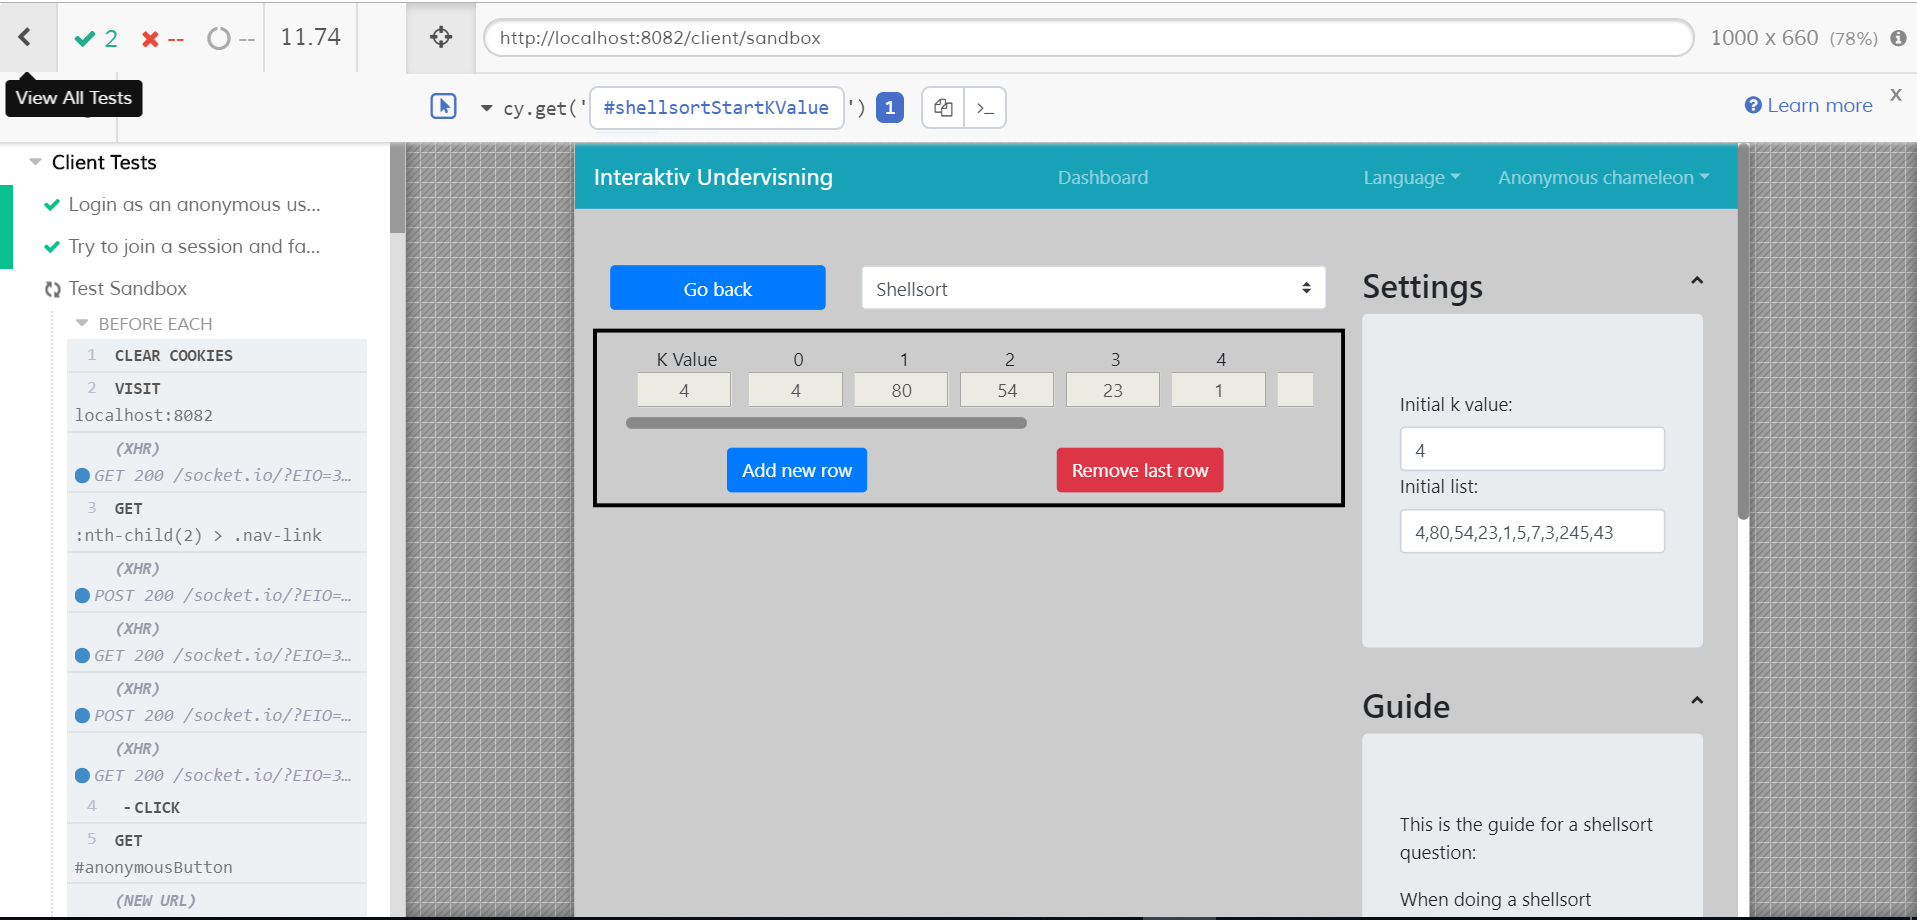
\includegraphics[width=0.90\linewidth]{/cypress}
	\caption{The figure displays the cypress testing tool.}
	\label{fig:cypress}
\end{figure}